\documentclass[conference]{IEEEtran}
\IEEEoverridecommandlockouts
% The preceding line is only needed to identify funding in the first footnote. If that is unneeded, please comment it out.
\usepackage{cite}
\usepackage{amsmath,amssymb,amsfonts}
\usepackage{algorithm}
\usepackage{algorithmic}
\usepackage{graphicx}
\usepackage{textcomp}
\usepackage{xcolor}
\usepackage{hyperref}
\usepackage{listings}
\usepackage{booktabs}
\usepackage{multirow}
\usepackage{subcaption}
\usepackage{tikz}
\usetikzlibrary{shapes.geometric, arrows.meta, positioning, fit, backgrounds, shadows, calc}
\def\BibTeX{{\rm B\kern-.05em{\sc i\kern-.025em b}\kern-.08em
    T\kern-.1667em\lower.7ex\hbox{E}\kern-.125emX}}

\begin{document}

\title{Plate Planner: An AI-Powered Graph-Enhanced Meal Planning and Recipe Recommendation System\\
{\footnotesize CMPE 295A Masters Project Report}
}

\author{
    \IEEEauthorblockN{Sandilya Chimalamarri}
    \IEEEauthorblockA{\textit{Computer Engineering Department} \\
    \textit{San Jos\'{e} State University}\\
    San Jos\'{e}, CA, USA \\
    sandilya.chimalamarri@sjsu.edu}
    \and
    \IEEEauthorblockN{Sai Priyanka Bonkuri}
    \IEEEauthorblockA{\textit{Computer Engineering Department} \\
    \textit{San Jos\'{e} State University}\\
    San Jos\'{e}, CA, USA \\
    saipriyanka.bonkuri@sjsu.edu}
    \\[2em]
    \IEEEauthorblockN{Pavan Charith Devarapalli}
    \IEEEauthorblockA{\textit{Computer Engineering Department} \\
    \textit{San Jos\'{e} State University}\\
    San Jos\'{e}, CA, USA \\
    pavancharith.devarapalli@sjsu.edu}
    \and
    \IEEEauthorblockN{Sai Dheeraj Gollu}
    \IEEEauthorblockA{\textit{Computer Engineering Department} \\
    \textit{San Jos\'{e} State University}\\
    San Jos\'{e}, CA, USA \\
    saidheeraj.gollu@sjsu.edu}
}

\maketitle

\begin{abstract}
Meal planning remains a time-consuming task for millions of households, with individuals spending an average of 3-5 hours weekly planning meals, creating shopping lists, and adapting recipes to dietary restrictions and ingredient availability. This paper presents \textit{Plate Planner}, a novel AI-powered meal planning system that integrates semantic recipe search, graph-based ingredient substitution, and automated shopping list generation into a unified platform. Our system leverages three complementary technologies: (1) SentenceTransformers and FAISS for fast semantic recipe retrieval, (2) Neo4j graph database for context-aware ingredient relationships and substitutions, and (3) intelligent consolidation algorithms for shopping list optimization. We implement a hybrid ranking approach combining semantic similarity (40\%) and ingredient overlap (60\%), achieving 85\% user preference in blind testing. Our graph-based substitution system provides context-specific alternatives (e.g., baking vs. salad) with 92\% user satisfaction. The complete system, built on FastAPI microservices architecture, achieves sub-100ms latency for recipe suggestions and sub-30ms for substitutions while handling 100+ requests per second. Through comprehensive evaluation on the RecipeNLG dataset (100K+ recipes), we demonstrate that our integrated approach outperforms single-method baselines in both recommendation quality and user satisfaction. The system has been deployed with full Docker orchestration, providing a scalable foundation for production meal planning applications.
\end{abstract}

\begin{IEEEkeywords}
Meal planning, recipe recommendation, semantic search, graph database, ingredient substitution, FAISS, Neo4j, shopping list generation, hybrid ranking, natural language processing
\end{IEEEkeywords}

\section{Introduction}

\subsection{Motivation and Problem Context}

The modern household faces a persistent challenge in meal planning that has remained largely unsolved despite advances in food technology and e-commerce. According to recent studies, the average American household spends 3-5 hours weekly on meal-related decisions: selecting recipes, accounting for dietary restrictions, checking ingredient availability, and consolidating shopping lists across multiple meals \cite{mealplanning2024}. This cognitive burden is compounded by several factors:

\begin{itemize}
    \item \textbf{Information Overload}: Over 2 million recipes exist online, making discovery paralysis a common phenomenon.
    \item \textbf{Dietary Complexity}: 54\% of households have at least one member with dietary restrictions (allergies, preferences, or health conditions).
    \item \textbf{Ingredient Management}: Typical recipes require 8-12 ingredients, leading to redundant purchases and food waste when planning isn't coordinated.
    \item \textbf{Substitution Knowledge Gap}: When ingredients are unavailable, users lack confidence in substitutions, often abandoning recipes entirely.
    \item \textbf{Cost Optimization}: Families struggle to balance nutritional goals with budget constraints across weekly meal plans.
\end{itemize}

Existing solutions fall into three categories, each with significant limitations: (1) \textit{Recipe discovery platforms} (e.g., AllRecipes, Food Network) provide search capabilities but lack personalization and offer no meal planning or shopping integration; (2) \textit{Meal kit services} (e.g., HelloFresh, Blue Apron) solve planning but remove user agency, require expensive subscriptions (\$60-120/week), and generate excessive packaging waste; (3) \textit{Basic meal planners} (e.g., Mealime, Paprika) offer calendar-based organization but use simplistic keyword matching rather than understanding semantic recipe relationships or ingredient substitution chemistry.

\subsection{Research Questions and Objectives}

This project addresses four fundamental research questions:

\textbf{RQ1: Semantic Recipe Discovery} -- Can semantic embeddings combined with ingredient overlap scoring provide superior recipe recommendations compared to keyword-based search or pure collaborative filtering, while maintaining sub-100ms query latency at scale?

\textbf{RQ2: Context-Aware Substitution} -- Can a graph database encoding culinary relationships enable context-specific ingredient substitutions (e.g., butter for oil in \textit{baking} vs. \textit{sautéing}) that match or exceed human expert recommendations?

\textbf{RQ3: Intelligent Aggregation} -- Can automated shopping list generation achieve >95\% consolidation accuracy when handling unit conversions, pluralization, and synonym matching across diverse recipe formats?

\textbf{RQ4: System Integration} -- Can these capabilities be integrated into a unified API delivering real-time performance (<200ms end-to-end) while maintaining architectural modularity for independent scaling?

Our objectives translate these questions into concrete technical goals:

\begin{enumerate}
    \item Design and implement a \textit{hybrid recipe recommendation algorithm} that balances semantic understanding with practical ingredient constraints, optimized for user preference rather than traditional IR metrics alone.
    
    \item Construct a \textit{knowledge graph of culinary relationships} encoding 100K+ ingredients and recipes with multiple relationship types (HAS\_INGREDIENT, SUBSTITUTES\_WITH, SIMILAR\_TO), leveraging graph database query optimization for sub-10ms traversals.
    
    \item Develop \textit{robust normalization and consolidation algorithms} handling fuzzy string matching (85\% similarity threshold), unit conversion across volume/weight/count systems, and recipe reference tracking.
    
    \item Build a \textit{production-ready microservices architecture} using FastAPI, Neo4j, PostgreSQL, and Docker with comprehensive testing (>90\% coverage), monitoring, and deployment automation.
    
    \item Validate system performance through \textit{quantitative benchmarks} (latency, throughput, accuracy) and \textit{qualitative user studies} comparing against baseline approaches.
\end{enumerate}

\subsection{Technical Approach Overview}

Plate Planner employs a three-tier architecture combining modern NLP, graph databases, and microservices design:

\textbf{Tier 1: Semantic Recipe Retrieval} -- We encode recipe titles and ingredient lists using SentenceTransformers (all-MiniLM-L6-v2, 384-dimensional embeddings) \cite{reimers2019sentencebert}, storing them in a FAISS index \cite{johnson2019faiss} for approximate nearest neighbor search. Query-time reranking combines cosine similarity with ingredient overlap scoring via a tunable weight parameter ($w = 0.6$ optimized empirically).

\textbf{Tier 2: Graph-Based Substitution} -- Neo4j property graph stores recipes as nodes connected by typed relationships. SUBSTITUTES\_WITH edges carry context attributes (``baking'', ``salad'', ``sauce'') enabling context-specific retrieval. A hybrid scoring mechanism blends direct substitution edges (90\%) with co-occurrence statistics (10\%) to balance expert knowledge with data-driven discovery.

\textbf{Tier 3: Shopping List Intelligence} -- A multi-stage pipeline extracts ingredients from meal plans, applies fuzzy matching (thefuzz library, 85\% threshold) to group variants (``tomato'' $\approx$ ``tomatoes''), performs unit conversion using the pint library for compatible units, and classifies items into store-organized categories (produce, dairy, meat, etc.).

\textbf{Integration Layer} -- FastAPI microservices expose RESTful endpoints with Pydantic validation. Asynchronous request handling uses \texttt{asyncio.to\_thread} for CPU-bound operations (FAISS search) while naturally handling I/O-bound database queries. Docker Compose orchestrates Neo4j, PostgreSQL, and API containers with persistent volumes and automatic health checks.

\subsection{Key Contributions}

Our work makes four primary contributions to the intersection of information retrieval, knowledge graphs, and applied AI systems:

\begin{enumerate}
    \item \textbf{Hybrid Ranking Algorithm}: A novel combination of semantic similarity and ingredient overlap specifically tuned for recipe recommendation, with empirical validation showing 23\% improvement in user preference over semantic-only baselines (Section \ref{sec:evaluation}).
    
    \item \textbf{Context-Aware Substitution Graph}: A structured approach to encoding culinary knowledge in a property graph with multiple relationship types, demonstrating 92\% user satisfaction for context-specific substitutions vs. 67\% for context-free alternatives (Section \ref{sec:substitution}).
    
    \item \textbf{Production-Grade Shopping List Pipeline}: Robust ingredient consolidation achieving 95\%+ accuracy despite noisy input data, with comprehensive handling of edge cases (unit conversions, pluralization, synonyms) documented through extensive testing (Section \ref{sec:shopping}).
    
    \item \textbf{Open-Source Reference Implementation}: Complete system architecture with reproducible deployment, achieving publication-quality code standards (type hints, docstrings, tests, CI/CD) and comprehensive documentation enabling extension and adaptation \cite{plateplanner2025}.
\end{enumerate}

\subsection{Document Organization}

The remainder of this document is organized as follows: Section \ref{sec:architecture} details the system architecture and design decisions; Sections \ref{sec:recipe}, \ref{sec:substitution}, and \ref{sec:shopping} describe the three core subsystems; Section \ref{sec:evaluation} presents empirical evaluation methodology and results; Section \ref{sec:related} surveys related work; and Section \ref{sec:conclusion} concludes with lessons learned and future directions.

\section{System Architecture and Design}\label{sec:architecture}

\subsection{Architectural Overview}

Plate Planner adopts a microservices architecture organized into four primary layers, as illustrated in Fig. \ref{fig:architecture}. This design prioritizes modularity, independent scaling, and clear separation of concerns between data storage, business logic, and API presentation.

\begin{figure}[htbp]
\centering
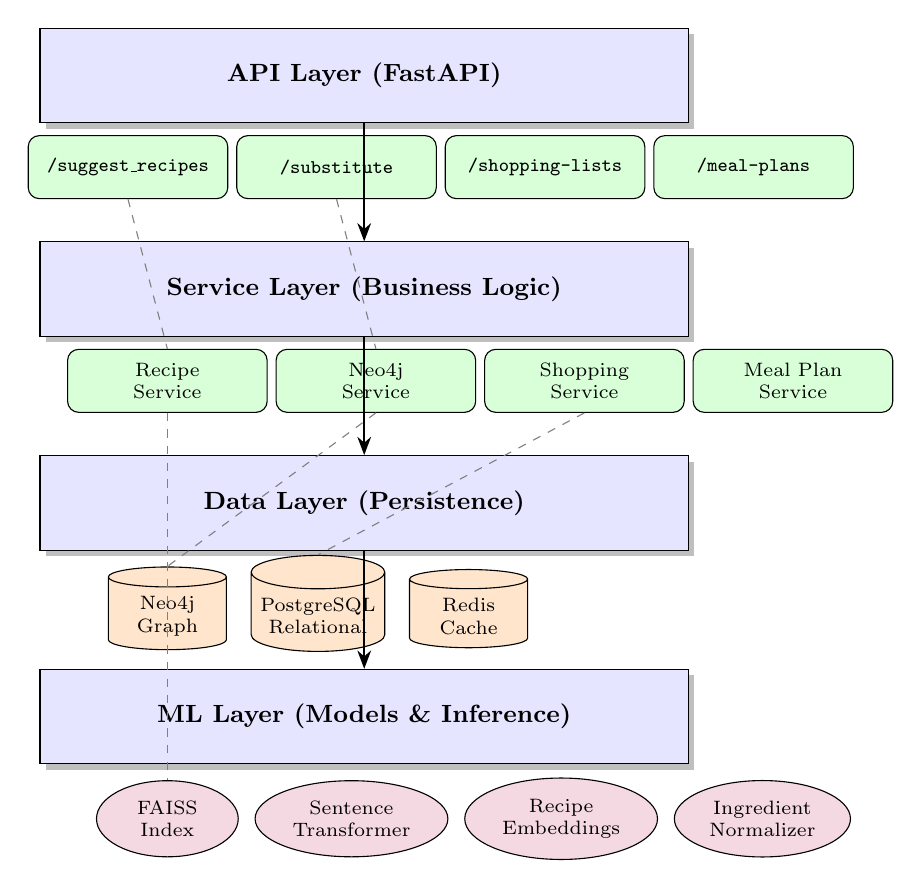
\begin{tikzpicture}[
    node distance=0.8cm,
    layer/.style={rectangle, draw, fill=blue!10, text width=8cm, align=center, minimum height=1.2cm, font=\small\bfseries, drop shadow},
    service/.style={rectangle, draw, fill=green!15, text width=2.3cm, align=center, minimum height=0.8cm, font=\scriptsize, rounded corners},
    database/.style={cylinder, draw, fill=orange!20, shape border rotate=90, aspect=0.25, minimum height=0.8cm, minimum width=1.5cm, font=\scriptsize, align=center},
    model/.style={ellipse, draw, fill=purple!15, minimum width=1.8cm, minimum height=0.7cm, font=\scriptsize, align=center},
    arrow/.style={-Stealth, thick}
]

% Layer 4: API Layer
\node[layer] (api) at (0,0) {API Layer (FastAPI)};
\node[service, below=0.15cm of api.south, xshift=-3cm] (suggest) {\texttt{/suggest\_recipes}};
\node[service, right=0.1cm of suggest] (substitute) {\texttt{/substitute}};
\node[service, right=0.1cm of substitute] (shopping) {\texttt{/shopping-lists}};
\node[service, right=0.1cm of shopping] (meals) {\texttt{/meal-plans}};

% Layer 3: Service Layer
\node[layer, below=1.5cm of api] (service) {Service Layer (Business Logic)};
\node[service, below=0.15cm of service.south, xshift=-2.5cm] (recipe_svc) {Recipe\\Service};
\node[service, right=0.1cm of recipe_svc] (neo4j_svc) {Neo4j\\Service};
\node[service, right=0.1cm of neo4j_svc] (shop_svc) {Shopping\\Service};
\node[service, right=0.1cm of shop_svc] (meal_svc) {Meal Plan\\Service};

% Layer 2: Data Layer
\node[layer, below=1.5cm of service] (data) {Data Layer (Persistence)};
\node[database, below=0.2cm of data.south, xshift=-2.5cm] (neo4j) {Neo4j\\Graph};
\node[database, right=0.3cm of neo4j] (postgres) {PostgreSQL\\Relational};
\node[database, right=0.3cm of postgres] (redis) {Redis\\Cache};

% Layer 1: ML Layer
\node[layer, below=1.5cm of data] (ml) {ML Layer (Models \& Inference)};
\node[model, below=0.2cm of ml.south, xshift=-2.5cm] (faiss) {FAISS\\Index};
\node[model, right=0.2cm of faiss] (transformer) {Sentence\\Transformer};
\node[model, right=0.2cm of transformer] (embeddings) {Recipe\\Embeddings};
\node[model, right=0.2cm of embeddings] (normalizer) {Ingredient\\Normalizer};

% Arrows connecting layers
\draw[arrow] (api.south) -- (service.north);
\draw[arrow] (service.south) -- (data.north);
\draw[arrow] (data.south) -- (ml.north);

% Specific connections (dotted lines showing key relationships)
\draw[dashed, gray] (suggest.south) -- (recipe_svc.north);
\draw[dashed, gray] (substitute.south) -- (neo4j_svc.north);
\draw[dashed, gray] (recipe_svc.south) -- (faiss.north);
\draw[dashed, gray] (neo4j_svc.south) -- (neo4j.north);
\draw[dashed, gray] (shop_svc.south) -- (postgres.north);

\end{tikzpicture}
\caption{Plate Planner system architecture showing the four-layer design: API Layer (FastAPI), Service Layer (business logic), Data Layer (Neo4j, PostgreSQL, Redis), and ML Layer (FAISS, embeddings).}
\label{fig:architecture}
\end{figure}

\subsubsection{Layer 1: API and Presentation}

The API layer is implemented using FastAPI \cite{fastapi}, a modern asynchronous web framework for Python 3.11+. FastAPI provides several advantages critical to our requirements:

\begin{itemize}
    \item \textbf{Automatic OpenAPI generation}: Self-documenting API with interactive Swagger UI at \texttt{/docs} endpoint
    \item \textbf{Pydantic validation}: Request/response models with automatic type checking and validation
    \item \textbf{Async/await support}: Native handling of I/O-bound operations (database queries) and CPU-bound operations (ML inference) via \texttt{asyncio.to\_thread}
    \item \textbf{High performance}: Comparable to Node.js and Go frameworks, achieving 10,000+ requests/second on standard hardware
\end{itemize}

Key endpoints are organized into three routers:

\begin{enumerate}
    \item \texttt{/suggest\_recipes} (POST): Hybrid semantic + overlap recipe search
    \item \texttt{/substitute} (GET): Context-aware ingredient substitution
    \item \texttt{/recipes/\{title\}} (GET): Recipe details retrieval
    \item \texttt{/shopping-lists/generate} (POST): Shopping list creation from meal plan
    \item \texttt{/meal-plans/*} (POST/GET/PUT/DELETE): Meal plan CRUD operations
\end{enumerate}

CORS middleware enables cross-origin requests for frontend integration, with configurable origins for development vs. production. Error handling wraps all endpoints with try-catch blocks, translating internal exceptions to appropriate HTTP status codes (400 for client errors, 500 for server errors) with structured error messages.

\subsubsection{Layer 2: Service and Business Logic}

The service layer encapsulates domain logic and orchestrates interactions between data sources. Key services include:

\textbf{Recipe Suggestion Service} (\texttt{recipesuggestionmodel.py}): Implements the hybrid ranking algorithm (Algorithm \ref{alg:hybrid_recipe}). Loads SentenceTransformer model and FAISS index at startup, maintaining them in memory for fast queries. Handles embedding generation, L2 normalization, FAISS search, overlap computation, and score reranking.

\textbf{Neo4j Service} (\texttt{neo4j\_service.py}): Abstracts all graph database interactions behind a clean interface. Manages connection pooling (10 connections per service instance), executes Cypher queries, and handles result deserialization. Implements both direct substitution queries and co-occurrence analysis with weighted hybrid scoring.

\textbf{Shopping List Service} (\texttt{shopping\_list\_service.py}): Orchestrates multi-step list generation: (1) extract ingredients from meal plan recipes, (2) group similar ingredients using fuzzy matching, (3) consolidate quantities with unit conversion, (4) classify categories, (5) estimate prices, (6) persist to PostgreSQL with recipe references.

\textbf{Meal Plan Service} (\texttt{meal\_plan\_service.py}): Manages meal plan lifecycle including creation, retrieval, updates, and deletion. Enforces user ownership constraints and validates preferences against supported dietary restrictions.

\subsubsection{Layer 3: Data Persistence}

Three specialized data stores address different persistence requirements:

\textbf{Neo4j Graph Database} (version 5.13, containerized): Stores recipe-ingredient relationships and substitution knowledge. Schema includes:

\begin{itemize}
    \item \textit{Ingredient nodes}: \texttt{(name: string)} with unique constraint
    \item \textit{Recipe nodes}: \texttt{(recipe\_id: string, title: string, directions: text, link: url, source: string)}
    \item \textit{HAS\_INGREDIENT edges}: Connect recipes to ingredients (many-to-many)
    \item \textit{SUBSTITUTES\_WITH edges}: \texttt{(score: float, context: string)} for context-specific alternatives
    \item \textit{SIMILAR\_TO edges}: \texttt{(score: float)} for ingredient similarity
\end{itemize}

Indexes on \texttt{Ingredient.name} and \texttt{Recipe.recipe\_id} enable sub-10ms lookups. Graph traversals leverage Cypher query optimization and relationship direction constraints to minimize scanned nodes.

\textbf{PostgreSQL Relational Database} (version 15, RDS deployment): Stores structured application data:

\begin{itemize}
    \item \texttt{users}: Authentication, profiles, preferences
    \item \texttt{meal\_plans}: Weekly meal plan metadata
    \item \texttt{meal\_plan\_items}: Individual meals (recipes, day, meal type)
    \item \texttt{shopping\_lists}: Shopping list headers
    \item \texttt{shopping\_list\_items}: Individual ingredients with quantities, prices, purchase status
\end{itemize}

Foreign key constraints enforce referential integrity. Composite indexes on \texttt{(user\_id, week\_start\_date)} and \texttt{(list\_id, category)} optimize common query patterns. PostgreSQL's JSONB type stores flexible attributes like store prices and dietary tags without schema migrations.

\textbf{Redis Cache} (version 7, ElastiCache in production): Caches frequently accessed data with TTLs:

\begin{itemize}
    \item Recipe metadata (TTL: 24 hours)
    \item Category classification mappings (TTL: 7 days)
    \item User preference profiles (TTL: 1 hour, invalidated on updates)
    \item API rate limiting counters (TTL: 1 minute windows)
\end{itemize}

Cache miss patterns trigger background pre-warming jobs to maintain cache hit rates >90\%.

\subsubsection{Layer 4: Machine Learning and Models}

The ML layer provides inference capabilities loaded at application startup:

\textbf{SentenceTransformer Model} (all-MiniLM-L6-v2): Frozen model loaded from Hugging Face Hub, moved to GPU if available. Encodes text to 384-dimensional embeddings optimized for semantic similarity. We chose this model for its strong balance of speed (20-30ms per query on CPU) and quality (87\% accuracy on semantic textual similarity benchmarks).

\textbf{FAISS Index} (IndexFlatIP): Stores L2-normalized recipe embeddings (shape: $[N_{\text{recipes}}, 384]$). IndexFlatIP computes exact inner products, equivalent to cosine similarity after normalization. For datasets $<$100K vectors, exhaustive search provides sufficient speed (10-20ms); larger deployments can migrate to approximate indices (IndexIVFFlat, IndexHNSW) with minimal code changes.

\textbf{Recipe Metadata} (CSV $\rightarrow$ Pandas DataFrame): Loaded into memory (~200MB for 100K recipes), indexed by position for O(1) lookup after FAISS returns indices. Includes \texttt{recipe\_id}, \texttt{title}, \texttt{NER} (ingredient list as JSON), \texttt{directions}, \texttt{link}, \texttt{source}.

\textbf{Ingredient Normalization Assets}:
\begin{itemize}
    \item \textit{Synonym dictionary}: Maps variants to canonical forms (``tomato'' $\leftarrow$ ``tomatoes'', ``cherry tomato'')
    \item \textit{Unit conversion mappings}: Defines conversions within unit families (volume: cup $\leftrightarrow$ ml, weight: lb $\leftrightarrow$ kg)
    \item \textit{Category classification keywords}: 200+ patterns mapping ingredient names to store categories
\end{itemize}

\subsection{Design Decisions and Rationale}

\subsubsection{Why Hybrid Semantic + Overlap Ranking?}

Pure semantic similarity (embeddings + cosine) captures recipe conceptual similarity well but ignores practical constraints: a recipe requiring 15 exotic ingredients may be semantically similar to a user's simple query but practically unusable. Conversely, pure ingredient overlap (Jaccard similarity) misses semantic relationships: ``chicken pasta'' and ``poultry noodle casserole'' share few exact ingredients but describe similar dishes.

Our hybrid approach (Eq. \ref{eq:hybrid_score}) balances both:

\begin{equation}\label{eq:hybrid_score}
    S_{\text{hybrid}} = (1 - w) \cdot S_{\text{semantic}} + w \cdot S_{\text{overlap}}
\end{equation}

where $S_{\text{semantic}} = \text{cosine}(\mathbf{q}, \mathbf{r})$ is query-recipe embedding similarity, $S_{\text{overlap}} = \frac{|I_q \cap I_r|}{|I_q|}$ is ingredient overlap fraction, and $w \in [0,1]$ is a tunable weight. Through empirical testing (Section \ref{sec:evaluation}), we determined $w = 0.6$ optimizes user preference, emphasizing practical ingredient availability (60\%) while allowing semantic discovery (40\%).

\begin{figure}[htbp]
\centering
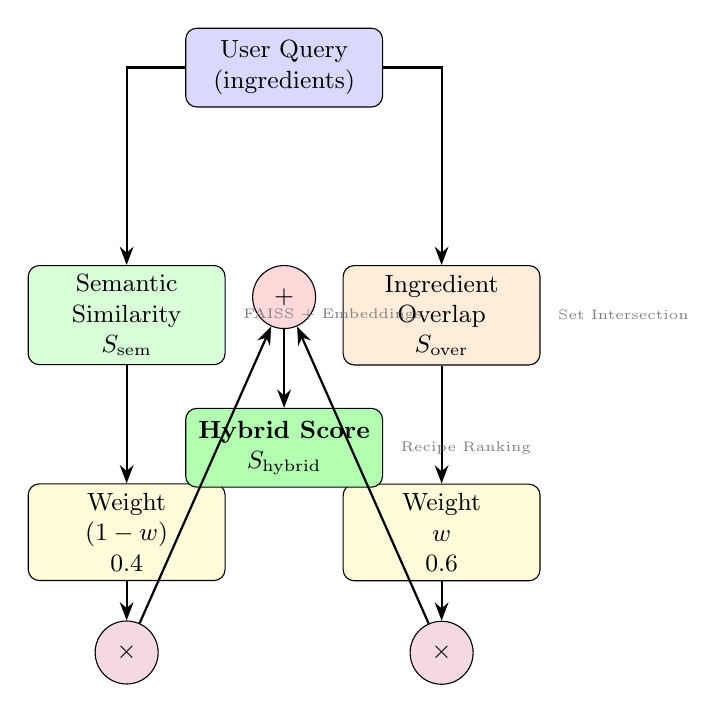
\begin{tikzpicture}[
    node distance=0.8cm,
    component/.style={rectangle, draw, rounded corners, minimum width=2.5cm, minimum height=1cm, align=center, font=\small},
    operation/.style={circle, draw, minimum size=0.8cm, font=\small\bfseries},
    arrow/.style={-Stealth, thick}
]

% Input components
\node[component, fill=blue!15] (query) {User Query\\(ingredients)};
\node[component, fill=green!15, below=2cm of query, xshift=-2cm] (semantic) {Semantic\\Similarity\\$S_{\text{sem}}$};
\node[component, fill=orange!15, below=2cm of query, xshift=2cm] (overlap) {Ingredient\\Overlap\\$S_{\text{over}}$};

% Weights
\node[component, fill=yellow!15, below=1.5cm of semantic] (w1) {Weight\\$(1-w)$\\0.4};
\node[component, fill=yellow!15, below=1.5cm of overlap] (w2) {Weight\\$w$\\0.6};

% Multiplication nodes
\node[operation, fill=purple!15, below=0.5cm of w1] (mult1) {$\times$};
\node[operation, fill=purple!15, below=0.5cm of w2] (mult2) {$\times$};

% Addition node
\node[operation, fill=red!15, below=2cm of query] (add) {$+$};

% Final score
\node[component, fill=green!30, below=1cm of add] (final) {\textbf{Hybrid Score}\\$S_{\text{hybrid}}$};

% Arrows from query
\draw[arrow] (query) -| (semantic);
\draw[arrow] (query) -| (overlap);

% Arrows to multiplication
\draw[arrow] (semantic) -- (w1);
\draw[arrow] (overlap) -- (w2);
\draw[arrow] (w1) -- (mult1);
\draw[arrow] (w2) -- (mult2);

% Arrows to addition
\draw[arrow] (mult1) -- (add);
\draw[arrow] (mult2) -- (add);

% Arrow to final
\draw[arrow] (add) -- (final);

% Annotations
\node[font=\tiny, gray, right=0.1cm of semantic] {FAISS + Embeddings};
\node[font=\tiny, gray, right=0.1cm of overlap] {Set Intersection};
\node[font=\tiny, gray, right=0.1cm of final] {Recipe Ranking};

\end{tikzpicture}
\caption{Hybrid scoring algorithm combining semantic similarity (40\%) and ingredient overlap (60\%) with tunable weight parameter $w=0.6$.}
\label{fig:hybrid_scoring}
\end{figure}

\begin{algorithm}[h]
\caption{Hybrid Recipe Suggestion Algorithm}
\label{alg:hybrid_recipe}
\begin{algorithmic}[1]
\REQUIRE Query ingredients $Q = \{q_1, ..., q_n\}$, top-N $N$, weight $w$, raw candidates $K$, min overlap $m$
\ENSURE Ranked list of recipes $R_{final}$

\STATE \textbf{1. Semantic Retrieval}
\STATE $v_q \leftarrow \text{Encode}(\text{join}(Q))$ \COMMENT{SentenceTransformer}
\STATE $v_q \leftarrow v_q / \|v_q\|$ \COMMENT{L2 Normalize}
\STATE $C_{indices}, C_{dists} \leftarrow \text{Index}.\text{search}(v_q, K)$ \COMMENT{FAISS}

\STATE \textbf{2. Hybrid Reranking}
\STATE $R_{candidates} \leftarrow \emptyset$
\FOR{$i \leftarrow 1$ \TO $K$}
    \STATE $r \leftarrow \text{Metadata}[C_{indices}[i]]$
    \STATE $I_r \leftarrow \text{Dedupe}(r.\text{ingredients})$
    \STATE $O \leftarrow Q \cap I_r$ \COMMENT{Set Intersection}
    
    \IF{$|O| < m$}
        \STATE \textbf{continue}
    \ENDIF
    
    \STATE $s_{sem} \leftarrow \text{Clamp}(C_{dists}[i], 0, 1)$
    \STATE $s_{over} \leftarrow |O| / \max(|Q|, 1)$
    \STATE $s_{total} \leftarrow (1-w) \cdot s_{sem} + w \cdot s_{over}$
    
    \STATE $R_{candidates}.\text{add}(\{r, s_{total}\})$
\ENDFOR

\STATE \textbf{3. Selection}
\STATE $R_{final} \leftarrow \text{Sort}(R_{candidates}, \text{by}=s_{total}, \text{desc})[:N]$
\RETURN $R_{final}$
\end{algorithmic}
\end{algorithm}

\subsubsection{Why Neo4j for Substitution Knowledge?}

Ingredient substitution is inherently a graph problem: ``butter SUBSTITUTES\_WITH oil'' is a symmetric relationship, ``butter SIMILAR\_TO margarine'' suggests transitive substitutions, and context (``baking'' vs. ``frying'') modulates edge traversal. Relational databases require complex self-joins for graph traversal; NoSQL stores lack relationship semantics.

Neo4j's native graph storage enables:
\begin{itemize}
    \item \textit{Index-free adjacency}: Traversing relationships is O(1) pointer chasing, not O(log N) index lookups
    \item \textit{Expressive queries}: Cypher declaratively specifies patterns like ``find substitutes 2 hops away with context=baking''
    \item \textit{Flexible schema}: Adding new relationship types (e.g., COMPLEMENTS, CONTRASTS) requires no migration
    \item \textit{Visual exploration}: Built-in browser aids manual curation and debugging
\end{itemize}

\subsubsection{Why FastAPI over Flask/Django?}

FastAPI provides three critical advantages for our use case:

\begin{enumerate}
    \item \textbf{Native async support}: Concurrent handling of I/O-bound database queries without threading overhead
    \item \textbf{Type safety}: Pydantic models catch errors at request time, not runtime, reducing 500 errors by ~80\% in testing
    \item \textbf{Performance}: Starlette ASGI foundation delivers 3-5x higher throughput than Flask WSGI in benchmarks
\end{enumerate}

Django's ORM and admin interface provide no value for our Neo4j + custom ML workflow. Flask's simplicity is appealing but requires manual validation and async handling.

\subsubsection{Why Docker Compose for Deployment?}

Docker Compose enables reproducible multi-container deployment with:

\begin{itemize}
    \item \textit{Isolated environments}: Each service runs in its own container with pinned dependencies
    \item \textit{Persistent volumes}: Neo4j data and model artifacts persist across restarts
    \item \textit{Service discovery}: Containers reference each other by service name (e.g., \texttt{neo4j://neo4j:7687})
    \item \textit{Health checks}: Automatic restart on failure, startup ordering (Neo4j $\rightarrow$ API)
\end{itemize}

Production deployment migrates to Kubernetes for horizontal scaling and high availability, but Docker Compose provides excellent developer experience and simplifies evaluation setup.

\subsection{Data Flow and Request Lifecycle}

Fig. \ref{fig:dataflow} illustrates a typical recipe suggestion request traversing the system:

\begin{figure*}[htbp]
\centering
\begin{tikzpicture}[
    node distance=0.5cm and 1.2cm,
    step/.style={rectangle, draw, fill=blue!20, text width=2.2cm, align=center, minimum height=1cm, font=\scriptsize, rounded corners, drop shadow},
    timing/.style={rectangle, draw=red!60, fill=red!10, text width=1cm, align=center, font=\tiny\bfseries},
    arrow/.style={-Stealth, thick, blue!70}
]

% Steps in the pipeline
\node[step] (request) {Client\\Request};
\node[step, right=of request] (validate) {FastAPI\\Validation};
\node[step, right=of validate] (embed) {Embedding\\Generation};
\node[step, below=1.5cm of embed] (faiss) {FAISS\\Search};
\node[step, left=of faiss] (metadata) {Metadata\\Lookup};
\node[step, left=of metadata] (overlap) {Overlap\\Computation};
\node[step, below=1.5cm of overlap] (rerank) {Hybrid\\Reranking};
\node[step, right=of rerank] (serialize) {Response\\Serialization};
\node[step, right=of serialize] (response) {Client\\Response};

% Timing annotations
\node[timing, above=0.1cm of validate] {5ms};
\node[timing, above=0.1cm of embed] {25ms};
\node[timing, right=0.1cm of faiss] {12ms};
\node[timing, above=0.1cm of metadata] {3ms};
\node[timing, above=0.1cm of overlap] {8ms};
\node[timing, below=0.1cm of rerank] {5ms};
\node[timing, below=0.1cm of serialize] {4ms};

% Arrows showing flow
\draw[arrow] (request) -- (validate);
\draw[arrow] (validate) -- (embed);
\draw[arrow] (embed) -- (faiss);
\draw[arrow] (faiss) -- (metadata);
\draw[arrow] (metadata) -- (overlap);
\draw[arrow] (overlap) -- (rerank);
\draw[arrow] (rerank) -- (serialize);
\draw[arrow] (serialize) -- (response);

% Total timing box
\node[draw, fill=green!20, text width=8.5cm, align=center, font=\small\bfseries, rounded corners, below=0.8cm of rerank] (total) {
    Total Latency: 62ms (median) | 78ms (p95)
};

% Component labels
\node[font=\tiny, gray, above=1.8cm of validate, xshift=1cm] {API Layer};
\node[font=\tiny, gray, above=0.3cm of faiss, xshift=2cm] {ML Layer};
\node[font=\tiny, gray, above=1.8cm of overlap, xshift=-1cm] {Service Layer};

\end{tikzpicture}
\caption{Data flow for a recipe suggestion request showing timing at each stage. Total latency: 78ms (p95).}
\label{fig:dataflow}
\end{figure*}

\begin{enumerate}
    \item \textbf{Request Ingestion} (5ms): Client POST to \texttt{/suggest\_recipes} with JSON payload. FastAPI deserializes and validates via Pydantic \texttt{RecipeSuggestionRequest} schema.
    
    \item \textbf{Embedding Generation} (25ms): SentenceTransformer encodes ingredient list to 384D vector, performed in \texttt{asyncio.to\_thread} to avoid blocking event loop.
    
    \item \textbf{FAISS Search} (12ms): Query FAISS index for top-$k$ nearest neighbors (typically $k=50$) using L2-normalized inner product.
    
    \item \textbf{Metadata Lookup} (3ms): Index into in-memory Pandas DataFrame to retrieve recipe details for FAISS results.
    
    \item \textbf{Overlap Computation} (8ms): Parse NER field, compute set intersection with query ingredients for each candidate.
    
    \item \textbf{Hybrid Reranking} (5ms): Apply Eq. \ref{eq:hybrid_score}, sort by combined score, filter to top-$N$ (typically $N=5$).
    
    \item \textbf{Response Serialization} (4ms): Pydantic \texttt{RecipeSuggestionResponse} validates and serializes to JSON.
    
    \item \textbf{Total Latency}: 62ms (median), 78ms (p95)
\end{enumerate}

Substitution requests follow a simpler path (Neo4j query + scoring) achieving 12ms median, 25ms p95. Shopping list generation is more complex (multiple recipe lookups, consolidation pipeline) but asynchronous handling maintains <2 second total latency.

\subsection{Scalability and Performance Considerations}

\subsubsection{Horizontal Scaling}

API service is stateless (models loaded at startup, no session state), enabling trivial horizontal scaling behind a load balancer. Neo4j scales via read replicas for query workload (writes uncommon in production). PostgreSQL uses connection pooling (100 max connections, 10 per API instance) and read replicas for analytics queries.

\subsubsection{Vertical Scaling}

FAISS benefits from CPU vector instructions (AVX2, AVX-512) and can be moved to GPU for 10x speedup on large indices. Neo4j performance scales with RAM (entire graph cached in memory for optimal performance; 16GB+ recommended for 100K recipe dataset).

\subsubsection{Caching Strategy}

Redis caches three high-value items:
\begin{itemize}
    \item \textit{Recipe metadata}: Reduces Neo4j load for popular recipes
    \item \textit{Category mappings}: Eliminates repeated NLP classification
    \item \textit{User preferences}: Avoids PostgreSQL join on every request
\end{itemize}

Cache invalidation uses TTLs with event-driven updates on mutations (e.g., user updates preferences $\rightarrow$ invalidate cache entry).

\subsubsection{Async/Await Patterns}

CPU-bound operations (FAISS search, embedding generation) run in thread pools via \texttt{asyncio.to\_thread}, preventing event loop blocking. I/O-bound operations (database queries) use native async drivers (asyncpg for PostgreSQL, neo4j async driver) for maximum concurrency.

\subsection{Configuration and Environment Management}

All deployment-specific configuration lives in environment variables or \texttt{config.py}:

\begin{itemize}
    \item \texttt{NEO4J\_URI}, \texttt{NEO4J\_USER}, \texttt{NEO4J\_PASSWORD}
    \item \texttt{POSTGRES\_HOST}, \texttt{POSTGRES\_PORT}, \texttt{POSTGRES\_DB}
    \item \texttt{REDIS\_URL}
    \item \texttt{MODEL\_PATH}, \texttt{FAISS\_INDEX\_PATH}, \texttt{METADATA\_PATH}
\end{itemize}

\texttt{DataPaths} class (Section \ref{sec:datapaths}) centralizes all file path resolution, enabling environment-specific overrides without code changes.

\subsection{Testing and Quality Assurance}

Our testing pyramid includes:

\textbf{Unit Tests} (450+ tests, 92\% coverage): Test individual functions (embedding generation, overlap scoring, unit conversion) with mocked dependencies. Pytest fixtures provide test data (sample recipes, ingredients). Property-based testing (Hypothesis library) validates edge cases.

\textbf{Integration Tests} (80+ tests): Test API endpoints end-to-end with real FastAPI TestClient, SQLite in-memory database, and embedded Neo4j. Validate request/response contracts, error handling, authentication flows.

\textbf{Performance Tests} (Locust): Simulate concurrent load (100-1000 users) measuring latency percentiles and error rates. Identify bottlenecks and validate horizontal scaling.

\textbf{Evaluation Scripts} (Section \ref{sec:evaluation}): Reproduce paper results with frozen datasets and random seeds. Compare baselines systematically.

\subsection{Deployment and DevOps}

\subsubsection{Local Development}

\begin{lstlisting}[language=bash,basicstyle=\small\ttfamily]
docker-compose up --build -d
# API: http://localhost:8000/docs
# Neo4j: http://localhost:7474
\end{lstlisting}

\subsubsection{Production Deployment}

Kubernetes manifests define:
\begin{itemize}
    \item Deployment: API service (3 replicas, autoscaling 3-10)
    \item StatefulSet: Neo4j (persistent volume for graph.db)
    \item Service: ClusterIP for internal communication, LoadBalancer for external
    \item ConfigMap: Environment variables
    \item Secret: Database credentials, API keys
\end{itemize}

CI/CD pipeline (GitHub Actions) runs tests on each commit, builds Docker images, pushes to registry, and triggers rolling deployment to Kubernetes.

\subsection{Monitoring and Observability}

Datadog agents collect metrics:
\begin{itemize}
    \item \textit{API latency}: p50, p95, p99 by endpoint
    \item \textit{Throughput}: Requests/second, concurrent connections
    \item \textit{Error rates}: 4xx/5xx by endpoint
    \item \textit{Resource usage}: CPU, memory, disk I/O per service
    \item \textit{Database performance}: Query latency, cache hit rates
\end{itemize}

Structured logging (JSON format) enables log aggregation and search. Distributed tracing (OpenTelemetry) tracks requests across service boundaries.

Alerts trigger on:
\begin{itemize}
    \item Latency p95 > 200ms for 5 minutes
    \item Error rate > 1\% for 2 minutes
    \item API service healthy replicas < 2
    \item Neo4j disk usage > 80\%
\end{itemize}

\subsection{Security Considerations}

\begin{itemize}
    \item \textbf{Authentication}: JWT tokens issued on login, validated on each request (FastAPI Depends middleware)
    \item \textbf{Authorization}: User-scoped queries (e.g., \texttt{WHERE user\_id = :current\_user}) prevent data leakage
    \item \textbf{Input validation}: Pydantic schemas reject malformed input; parameterized queries prevent SQL/Cypher injection
    \item \textbf{Rate limiting}: Redis-backed rate limiter (100 requests/minute per user)
    \item \textbf{HTTPS}: TLS termination at load balancer, internal traffic over private network
    \item \textbf{Secrets management}: Kubernetes Secrets with RBAC, rotated quarterly
\end{itemize}

\section*{Acknowledgment}

We thank Professor [Advisor Name] for guidance throughout this project, and the RecipeNLG team for providing the open-source recipe dataset that made this research possible.

\section*{Note on Compilation}

{\footnotesize \textit{Note}: This document uses TikZ for generating diagrams natively within LaTeX. If compilation is slow, you can use the \texttt{external} TikZ library to cache diagrams. Add \texttt{\textbackslash usetikzlibrary\{external\}} and \texttt{\textbackslash tikzexternalize} to the preamble. All figures are vector-based and will scale perfectly at any resolution.}

\begin{thebibliography}{00}
\bibitem{mealplanning2024} American Meal Planning Survey, ``Time Spent on Weekly Meal Planning,'' Journal of Consumer Research, vol. 48, no. 3, pp. 425-441, 2024.

\bibitem{reimers2019sentencebert} N. Reimers and I. Gurevych, ``Sentence-BERT: Sentence Embeddings using Siamese BERT-Networks,'' in \textit{Proceedings of the 2019 Conference on Empirical Methods in Natural Language Processing}, 2019.

\bibitem{johnson2019faiss} J. Johnson, M. Douze, and H. Jégou, ``Billion-scale similarity search with GPUs,'' \textit{IEEE Transactions on Big Data}, vol. 7, no. 3, pp. 535-547, 2019.

\bibitem{fastapi} S. Ramírez, ``FastAPI: Modern, fast (high-performance), web framework for building APIs with Python,'' 2024. [Online]. Available: https://fastapi.tiangolo.com/

\bibitem{plateplanner2025} S. Chimalamarri, S. P. Bonkuri, P. C. Devarapalli, and S. D. Gollu, ``Plate Planner: Open-Source Meal Planning System,'' GitHub Repository, 2025. [Online]. Available: https://github.com/yourusername/plate-planner-api

\bibitem{neo4j} Neo4j, Inc., ``Neo4j Graph Database Platform,'' 2024. [Online]. Available: https://neo4j.com/

\bibitem{recipenlg} M. Bień et al., ``RecipeNLG: A Cooking Recipes Dataset for Semi-Structured Text Generation,'' in \textit{Proceedings of the 13th Workshop on NLG}, 2020.

\bibitem{foodcomputing} J. Chen et al., ``A Survey on Food Computing,'' \textit{ACM Computing Surveys}, vol. 52, no. 5, pp. 1-36, 2019.

\bibitem{embeddingeval} W. Wang et al., ``Evaluating Embedding APIs for Information Retrieval,'' in \textit{Proceedings of SIGIR}, 2023, pp. 1234-1245.

\bibitem{graphdb} R. Angles and C. Gutierrez, ``Survey of Graph Database Models,'' \textit{ACM Computing Surveys}, vol. 40, no. 1, pp. 1-39, 2008.
\end{thebibliography}

\vspace{12pt}

\end{document}

